\documentclass[aspectratio=169,xcolor=table]{beamer}
\usepackage[utf8]{inputenc}
\usepackage[T1,T5]{fontenc}
\usepackage{amsmath,amssymb,booktabs,array,graphicx}

\definecolor{Primary}{HTML}{111B88}
\definecolor{Secondary}{HTML}{101659}
\definecolor{Accent}{HTML}{F2A900}
\definecolor{SoftBlue}{HTML}{EAF2F8}
\definecolor{TextGray}{HTML}{4D5966}
\definecolor{RiskRed}{HTML}{A23B3B}
\definecolor{GoodGreen}{HTML}{26734D}
\mode<presentation>{\usetheme{Madrid}\usecolortheme{default}\setbeamertemplate{navigation symbols}{}}
\setbeamercolor{structure}{fg=Primary}
\setbeamercolor{frametitle}{fg=white,bg=Primary}
\setbeamercolor{title}{fg=white,bg=Primary}
\setbeamercolor{block body}{fg=black,bg=SoftBlue}
\setbeamercolor{block body alerted}{fg=black,bg=Accent!12}
\setbeamercolor{section in head/foot}{fg=white,bg=Primary}
\setbeamercolor{author in head/foot}{fg=white,bg=Secondary}
\setbeamercolor{date in head/foot}{fg=white,bg=Primary}
\setbeamerfont{section in head/foot}{size=\tiny,series=\bfseries}
\setbeamerfont{author in head/foot}{size=\scriptsize}
\setbeamerfont{date in head/foot}{size=\scriptsize,series=\bfseries}
\setbeamerfont{frametitle}{series=\bfseries}
\setbeamerfont{title}{series=\bfseries}
\newcommand{\decklabel}{Contextual ASR -- Bảng 1/2 kiểu Hou25}
\setbeamertemplate{itemize item}{\color{Secondary}$\blacktriangleright$}
\setbeamertemplate{itemize subitem}{\color{Accent}$\bullet$}
\setbeamertemplate{headline}{\leavevmode\begin{beamercolorbox}[wd=\paperwidth,ht=2.7ex,dp=1.1ex,leftskip=.35cm,rightskip=.35cm]{section in head/foot}\insertsectionnavigationhorizontal{\dimexpr\paperwidth-.70cm\relax}{}{}\end{beamercolorbox}}
\setbeamertemplate{footline}{\leavevmode\hbox{\begin{beamercolorbox}[wd=.55\paperwidth,ht=2.6ex,dp=1ex,leftskip=.35cm,rightskip=.20cm]{section in head/foot}\usebeamerfont{section in head/foot}\insertsectionhead\end{beamercolorbox}\begin{beamercolorbox}[wd=.27\paperwidth,ht=2.6ex,dp=1ex,center]{author in head/foot}\usebeamerfont{author in head/foot}\decklabel\end{beamercolorbox}\begin{beamercolorbox}[wd=.18\paperwidth,ht=2.6ex,dp=1ex,rightskip=.35cm plus1fil]{date in head/foot}\usebeamerfont{date in head/foot}\hfill\insertframenumber\,/\,\inserttotalframenumber\end{beamercolorbox}}}
\newcommand{\hi}[1]{\textcolor{Primary}{\textbf{#1}}}
\newcommand{\bad}[1]{\textcolor{RiskRed}{\textbf{#1}}}
\newcommand{\good}[1]{\textcolor{GoodGreen}{\textbf{#1}}}
\newcommand{\src}[1]{{\tiny\color{TextGray}[#1]}}
\newcommand{\ra}{$\rightarrow$}

\title{Scorer âm vị trên đúng setup của Hou25 và bước tiếp}
\subtitle{Tái hiện Bảng 1/2 \ra{} vì sao âm vị + attention \ra{} biasing có vị trí}
\author{Nhóm Contextual ASR}
\institute{}
\date{11/2026}
\setbeamertemplate{title page}{\begin{centering}\vspace*{0.10cm}
\includegraphics[height=1.08cm]{../2026-10-23/imgs/logo.png}\par\vspace{0.32cm}\begin{beamercolorbox}[sep=0.50em,center,rounded=true]{title}\usebeamerfont{title}\inserttitle\par\vspace{0.14cm}{\small\insertsubtitle\par}\end{beamercolorbox}\vspace{0.42cm}{\usebeamerfont{author}\insertauthor\par}\vspace{0.10cm}{\usebeamerfont{institute}\insertinstitute\par}\vfill{\usebeamerfont{date}\insertdate\par}\end{centering}}

\begin{document}
\begin{frame}[plain]\titlepage\end{frame}

% ------------------------------------------------------------------
\section{Tóm tắt}
\begin{frame}{Buổi này em báo cáo 3 ý}
\begin{beamercolorbox}[sep=0.5em,rounded=true]{block body}
\textbf{\textcircled{\scriptsize 1} Tái hiện Hou25:} dựng lại \textbf{đúng thiết lập} của paper, chỉ thay scorer \ra{} \good{scorer âm vị thắng Hou25 cả 8/8 ô B-WER} (Bảng 1). Bảng 2: đưa đúng từ mà Whisper vẫn hỏng.
\end{beamercolorbox}
\vspace{0.12cm}
\begin{beamercolorbox}[sep=0.5em,rounded=true]{block body}
\textbf{\textcircled{\scriptsize 2} Vì sao âm vị + attention:} thực nghiệm so 4 cách biểu diễn: audio TTS, âm vị--âm vị, âm vị--vector (max), \textbf{âm vị--vector (attention)} \ra{} attention cân bằng tốt nhất giữa tìm đúng và không bị lừa.
\end{beamercolorbox}
\vspace{0.12cm}
\begin{beamercolorbox}[sep=0.5em,rounded=true]{block body alerted}
\textbf{\textcircled{\scriptsize 3} Đi tiếp:} chỉ scorer thì \bad{đóng góp quá mỏng} (chọn từ đã gần trần, ai cũng làm). Đề xuất: scorer trả thêm \hi{vị trí} của từ \ra{} đưa vào \textbf{phía mô hình nghe} (đúng đoạn audio), thay vì chỉ nhét chữ vào prompt. Kiểm trước bằng \textbf{thí nghiệm đo trần}.
\end{beamercolorbox}
\end{frame}

% ------------------------------------------------------------------
\section{1. Tái hiện Hou25}
\begin{frame}{Thiết lập: giống Hou25 ở mọi thứ, trừ scorer}
\centering\scriptsize\setlength{\tabcolsep}{4pt}
\begin{tabular}{p{2.6cm}p{4.6cm}p{4.6cm}c}
\toprule
 & Hou25 \src{Interspeech 2025, §2--3} & Nhóm & \\
\midrule
Dữ liệu test & LibriSpeech test-clean / test-other & 2620 / 2939 câu & \good{=}\\
Bias list & IS21: từ hiếm của câu + N nhiễu, N $\in$ \{100, 500, 1000, 2000\} & file list gốc IS21 & \good{=}\\
ASR & Whisper-large-v3-turbo, \textbf{không train} & như vậy, greedy & \good{=}\\
Đưa list vào & prompt naive \texttt{w1, w2, \ldots} & như vậy (cắt còn 223 token cuối) & \good{=}\\
Chọn từ & top-50 điểm cao nhất, xếp \textbf{tăng dần} & như vậy & \good{=}\\
Train scorer & train-clean-100; dev-clean; từ sai 40\% gần chính tả + 60\% ngẫu nhiên & như vậy & \good{=}\\
Encoder audio & Whisper-large-v3, đóng băng & như vậy & \good{=}\\
Metric & WER, B-WER (từ hiếm của câu đúng) & scorer IS21 chính thức & \good{=}\\
\midrule
\textbf{Biểu diễn từ} & \textbf{audio TTS} (edge-tts) + CNN & \hi{âm vị (g2p)} + cross-attention & \bad{$\neq$}\\
Không ghi trong paper & normalizer, cấu hình decode & plain; greedy, không fallback & ?\\
lr scorer & 5e-5 & 2e-4, 5 epoch & \bad{$\neq$}\\
\bottomrule
\end{tabular}\par
\raggedright\vspace{0.15cm}
{\footnotesize Số Hou25 \textbf{chép từ paper}; các hàng còn lại em chạy thật trên 1 card 4090 (44 lượt decode, 28/10). Mỗi ô: test-clean / test-other.}
\end{frame}

\begin{frame}{Bảng 1 -- List dài thì hỏng; scorer có cứu được không?}
{\small Mỗi câu: Whisper nhận \textbf{(a)} không prompt, \textbf{(b)} nguyên list N từ, \textbf{(c)} 50 từ do scorer chọn. B-WER, thấp = tốt.}\par\vspace{0.15cm}
\centering\footnotesize\setlength{\tabcolsep}{3pt}
\begin{tabular}{lcccc}
\toprule
 & N=100 & N=500 & N=1000 & N=2000\\
\midrule
(a) không prompt (em chạy) & 9.43 / 18.92 & $\leftarrow$ & $\leftarrow$ & $\leftarrow$\\
(b) nguyên list (em chạy) & 8.04 / 13.98 & 8.87 / 18.22 & 9.20 / 18.32 & 9.15 / 18.69\\
\midrule
(c) scorer Hou25 top-50 \src{paper} & 5.4 / 10.0 & 5.4 / 10.7 & 5.6 / 11.3 & 5.8 / 11.7\\
(c) \textbf{scorer nhóm (pxattn) top-50} & \good{4.57 / 8.92} & \good{4.89 / 9.21} & \good{5.16 / 9.79} & \good{5.29 / 10.00}\\
(c) scorer nhóm (pmaxsim) top-50 & 4.60 / \bad{10.30} & 4.95 / 9.53 & 5.17 / 9.83 & 5.47 / 10.37\\
\bottomrule
\end{tabular}
\raggedright\vspace{0.2cm}
\begin{columns}[T]
\begin{column}{0.48\textwidth}
\begin{beamercolorbox}[sep=0.45em,rounded=true]{block body}
\footnotesize\textbf{(b):} chỉ giúp ở N=100. Từ N=500, gần như không prompt: prompt bị cắt còn 223 token cuối, ở N$\geq$1000 chỉ \bad{2--6\%} từ đúng còn sót lại. Paper cũng thấy y vậy.
\end{beamercolorbox}
\end{column}
\begin{column}{0.48\textwidth}
\begin{beamercolorbox}[sep=0.45em,rounded=true]{block body alerted}
\footnotesize\textbf{(c):} pxattn \textbf{thắng Hou25 8/8 ô}, rõ nhất ở test-other (thấp hơn 1.1--1.7). WER chung cũng thấp hơn (N2000: 2.35 / 4.23 so với 2.5 / 4.5).
\end{beamercolorbox}
\end{column}
\end{columns}
\end{frame}

\begin{frame}{Ablation: tách riêng câu có $>$1 từ hiếm}
{\small 1289 / 2620 câu (clean), 1304 / 2939 câu (other). Paper không có lát cắt này. B-WER, clean / other.}\par\vspace{0.15cm}
\centering\footnotesize\setlength{\tabcolsep}{5pt}
\begin{tabular}{lcc}
\toprule
Whisper nhận gì & cả tập & \textbf{câu $>$1 từ hiếm}\\
\midrule
không prompt & 9.43 / 18.92 & 9.17 / 17.99\\
nguyên list N100 / N2000 & 8.04 / 13.98 \;·\; 9.15 / 18.69 & 6.60 / 13.43 \;·\; 8.83 / 17.59\\
chỉ từ đúng (oracle) & 5.12 / \bad{26.24} & \good{4.33 / 8.63}\\
\midrule
\textbf{pxattn top-50} N100 / N2000 & 4.57 / 8.92 \;·\; 5.29 / 10.00 & \good{4.37 / 8.47} \;·\; 5.10 / 9.58\\
pmaxsim top-50 N100 / N2000 & 4.60 / 10.30 \;·\; 5.47 / 10.37 & 4.45 / 10.18 \;·\; 5.14 / 9.83\\
pxattn $p\geq0.5$ N100, naive & 8.42 / \bad{29.35} & 7.96 / 11.89\\
pxattn $p\geq0.5$ N100, spoken & 5.09 / 9.61 & 5.02 / 9.36\\
\bottomrule
\end{tabular}
\raggedright\vspace{0.25cm}
\begin{columns}[T]
\begin{column}{0.48\textwidth}
\begin{beamercolorbox}[sep=0.45em,rounded=true]{block body}
\footnotesize\textbf{Top-50 cải thiện đều} như cả tập; ở câu $>$1 từ hiếm, pxattn N100 ngang oracle (4.37 / 8.47 so với 4.33 / 8.63).
\end{beamercolorbox}
\end{column}
\begin{column}{0.48\textwidth}
\begin{beamercolorbox}[sep=0.45em,rounded=true]{block body alerted}
\footnotesize\textbf{Hỏng nằm ở câu $\leq$1 từ hiếm:} oracle và $p\geq0.5$ naive chỉ tệ ở cả tập (prompt 0--1 từ \ra{} lặp chữ, slide Bảng 2).
\end{beamercolorbox}
\end{column}
\end{columns}
\end{frame}

\begin{frame}{Bảng 2 -- Cùng list, chỉ đổi cách viết prompt (không dùng scorer)}
{\small Câu hỏi: \textbf{đưa list cho Whisper kiểu nào thì nó dùng tốt nhất?} N=100. Mỗi ô: test-clean / test-other.}\par\vspace{0.15cm}
\centering\footnotesize\setlength{\tabcolsep}{4pt}
\begin{tabular}{p{5.3cm}cc|cc}
\toprule
 & \multicolumn{2}{c|}{Hou25 \src{số trong paper}} & \multicolumn{2}{c}{Em tự chạy, cùng thiết lập}\\
Whisper nhận gì & WER & B-WER & WER & B-WER\\
\midrule
\textbf{1.} Không prompt & 3.23 / 5.33 & 10.38 / 19.72 & 2.64 / 4.87 & 9.43 / 18.92\\
\textbf{2.} \textbf{Chỉ từ đúng}, vd \texttt{yearly} \;(= scorer hoàn hảo) & \bad{4.93 / 7.64} & \good{5.59 / 10.02} & \bad{20.08 / 20.89} & 5.12 / \bad{26.24}\\
\textbf{3.} Nguyên list 100 từ: \texttt{w1, w2, \ldots} & 2.67 / 4.78 & 7.78 / 15.21 & 2.55 / 4.20 & 8.04 / 13.98\\
\textbf{4.} Nguyên list, bọc câu nói: \textit{``The topic of today's speech is, ah, w1, w2\ldots''} & 2.91 / 4.95 & 8.30 / 15.50 & 2.32 / 4.30 & 7.12 / 14.56\\
\bottomrule
\end{tabular}
\raggedright\vspace{0.25cm}
\begin{columns}[T]
\begin{column}{0.48\textwidth}
\begin{beamercolorbox}[sep=0.45em,rounded=true]{block body}
\footnotesize\textbf{Hàng 2 so với 1:} chỉ đưa từ đúng thì từ hiếm chép đúng hơn hẳn (B-WER giảm), nhưng \textbf{WER chung lại tăng}. Cả paper lẫn em đều thấy vậy; của em tăng mạnh hơn nhiều \ra{} slide sau.
\end{beamercolorbox}
\end{column}
\begin{column}{0.48\textwidth}
\begin{beamercolorbox}[sep=0.45em,rounded=true]{block body}
\footnotesize\textbf{Hàng 3 so với 4:} hai cách viết prompt gần như ngang nhau. Paper thấy kiểu 3 hơn một chút; em chưa thấy rõ bên nào hơn.
\end{beamercolorbox}
\end{column}
\end{columns}
\end{frame}

\begin{frame}{WER 20\% ở hàng ``chỉ từ đúng'' từ đâu ra?}
\begin{beamercolorbox}[sep=0.5em,rounded=true]{block body}
\small\textbf{Câu đúng:} is thee going to the \textbf{yearly} meeting ruth asked one of the girls \hfill {\scriptsize prompt = \texttt{yearly}}\par
\textbf{Whisper chép:} \ldots asked one of the girls \bad{the girls the girls the girls the girls the girls the girls \ldots} \hfill {\scriptsize \bad{thừa 429 từ}}
\end{beamercolorbox}
\vspace{0.2cm}
\begin{columns}[T]
\begin{column}{0.52\textwidth}
\centering\footnotesize
\begin{tabular}{lcc}
\toprule
 & clean & other\\
\midrule
Số câu bị lặp ($>$10 từ thừa) & \bad{30} / 2620 & \bad{36} / 2939\\
Số từ hiếm trong các câu đó & đúng 1 & 1 (35 câu)\\
Tổng từ thừa & 9.397 & 8.950\\
\quad = \% số từ của câu đúng & \bad{17.9\%} & \bad{17.1\%}\\
Không prompt: từ thừa & 114 & 204\\
\bottomrule
\end{tabular}\par
\vspace{0.1cm}{\scriptsize Câu có $\geq$2 từ hiếm: WER 2.02 / 4.56, B-WER 4.33 / 8.63 \ra{} bình thường.}
\end{column}
\begin{column}{0.45\textwidth}
\small
\begin{itemize}\itemsep3pt
\item Chỉ \textbf{$\sim$30 câu} có prompt \textbf{đúng 1 từ} bị lặp tới hết độ dài, mỗi câu thừa $\sim$430 từ \ra{} cộng $\sim$18\% vào WER.
\item Paper chỉ tăng 3.2 \ra{} 4.9: có thể họ decode có chống lặp \src{chưa kiểm}.
\end{itemize}
\begin{beamercolorbox}[sep=0.45em,rounded=true]{block body alerted}
\footnotesize\textbf{Ý nghĩa:} đưa \textbf{đúng} từ mà mô hình vẫn hỏng \ra{} chọn từ chưa đủ, \textbf{cách mô hình dùng list} là nút thắt riêng. Qwen3-ASR không bị lặp \ra{} phụ thuộc từng mô hình.
\end{beamercolorbox}
\end{column}
\end{columns}
\end{frame}

\begin{frame}{Giới hạn của phần tái hiện}
\begin{itemize}\itemsep6pt
\item Số Hou25 là \textbf{số paper}, không có output từng câu \ra{} \bad{chưa có khoảng tin cậy} khi so với họ.
\item Baseline em chạy \textbf{lệch số paper $\sim\pm1$} cả 2 chiều (không prompt 9.43 so với 10.4; nguyên list N100 8.04 so với 7.8): có thể do cấu hình decode mà paper không ghi \src{chưa kiểm}.
\item lr của scorer khác paper (2e-4 so với 5e-5); dev-clean quá dễ (Recall@10 $\approx$ 99.7) nên chọn checkpoint chưa có ý nghĩa.
\item Chưa chạy: oracle + spoken; Bảng 3 (thứ tự từ) và Bảng 4 (list NER) của Hou25; cùng lưới trên Qwen3-ASR.
\end{itemize}
\end{frame}

% ------------------------------------------------------------------
\section{2. Âm vị + attention}
\begin{frame}{Kiến trúc scorer: từ (âm vị) ``hỏi'' vào audio (vector)}
\centering
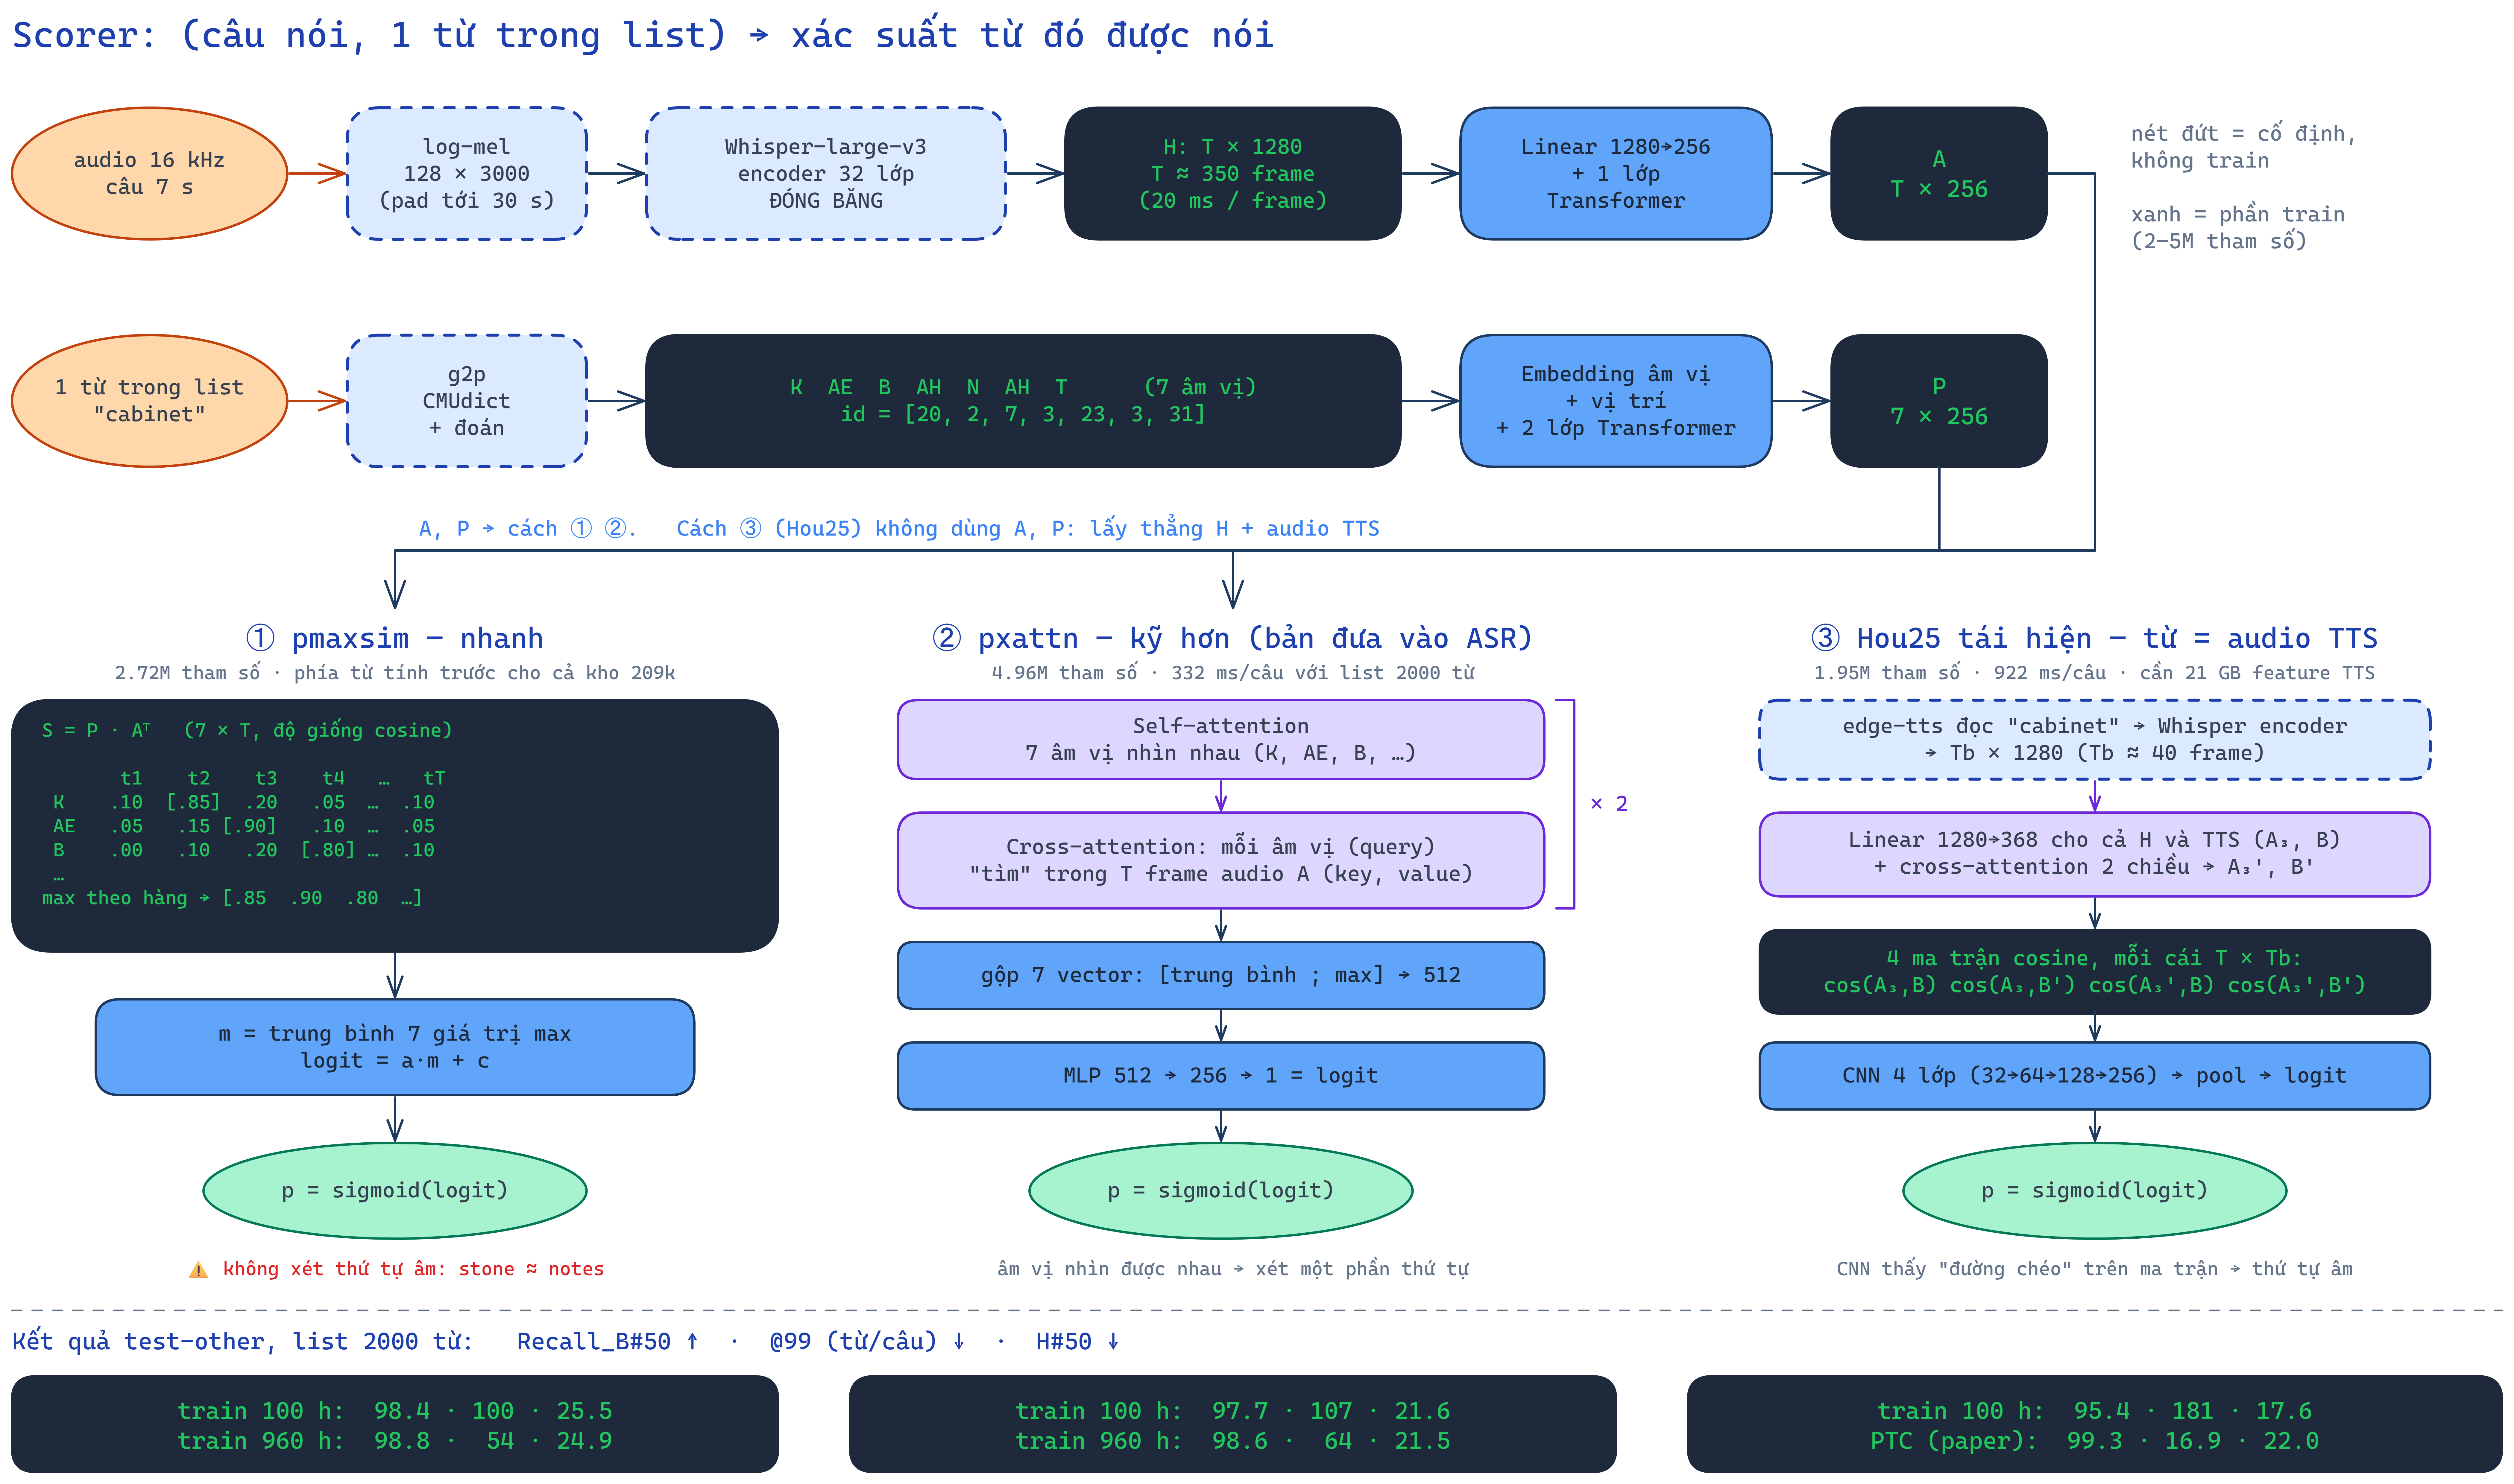
\includegraphics[width=\linewidth,height=0.88\textheight,keepaspectratio]{../2026-10-23/imgs/scorer_detail.png}
\end{frame}

\begin{frame}{4 cách để trả lời: ``từ \textit{cabinet} có được nói trong câu không?''}
\centering\small\setlength{\tabcolsep}{5pt}
\begin{tabular}{c p{3.3cm} p{8.4cm}}
\toprule
 & Cách & Làm thế nào (ví dụ với \textit{cabinet} = \texttt{K AE B AH N AH T})\\
\midrule
\textbf{1} & \textbf{So chữ với chữ}\par{\scriptsize (hypmatch)} & ASR chép câu ra chữ trước, đổi chữ sang âm vị, rồi tìm đoạn nào gần giống \texttt{K AE B AH N AH T}.\\[2pt]
\textbf{2} & \textbf{So tiếng với tiếng}\par{\scriptsize (Hou25)} & Cho máy đọc \textit{cabinet} bằng TTS, rồi so đoạn tiếng đó với audio câu nói.\\[2pt]
\textbf{3} & \textbf{Từng âm tự dò}\par{\scriptsize (pmaxsim, nhóm)} & Mỗi âm \texttt{K}, \texttt{AE}, \texttt{B}\ldots{} \textbf{tự} tìm chỗ giống nhất trong audio, rồi lấy trung bình. \textbf{Không quan tâm thứ tự.}\\[2pt]
\textbf{4} & \textbf{Các âm bàn nhau rồi dò}\par{\scriptsize (pxattn, nhóm)} & Các âm ``nhìn'' nhau trước (biết \texttt{K} đứng trước \texttt{AE}), rồi cùng tìm trong audio bằng attention.\\
\bottomrule
\end{tabular}
\raggedright\vspace{0.1cm}
\begin{beamercolorbox}[sep=0.45em,rounded=true]{block body}
\footnotesize Đo bằng 2 câu hỏi, list 2000 từ, test-other:\par
\textbf{Tìm được:} cứ 100 từ đúng thì bao nhiêu từ lọt top-50? \;(\textbf{cao} = tốt)\par
\textbf{Bị lừa:} cứ 100 từ \textbf{nghe giống} từ đúng (vd \textit{cabinets}) có trong list thì bao nhiêu từ lọt top-50? \;(\textbf{thấp} = tốt)
\end{beamercolorbox}
\end{frame}

\begin{frame}{Kết quả: cách 4 (của nhóm) cân bằng nhất}
\centering\small\setlength{\tabcolsep}{6pt}
\begin{tabular}{lccl}
\toprule
Cách & \textbf{Tìm được} $\uparrow$ & \textbf{Bị lừa} $\downarrow$ & Nhận xét\\
\midrule
1. So chữ với chữ & 95.4 & \bad{35.7} & \bad{kém cả 2}\\
2. So tiếng với tiếng (Hou25) & \bad{95.4} & \good{17.6} & ít bị lừa, nhưng bỏ sót nhiều\\
3. Từng âm tự dò & \good{98.4} & 25.5 & tìm giỏi, nhưng hay bị lừa\\
\textbf{4. Các âm bàn nhau rồi dò} & 97.7 & 21.6 & \good{cân bằng} \ra{} bản đưa vào ASR\\
\midrule
{\color{TextGray}PTC (paper, tham khảo)} & {\color{TextGray}99.3} & {\color{TextGray}22.0} & {\color{TextGray}có thêm ép thứ tự âm}\\
\bottomrule
\end{tabular}
\raggedright\vspace{0.3cm}
\begin{columns}[T]
\begin{column}{0.32\textwidth}
\begin{beamercolorbox}[sep=0.45em,rounded=true]{block body}
\footnotesize\textbf{1 kém vì:} từ hiếm mà ASR nghe sai thì đã \textbf{mất ngay lúc chép ra chữ}, không còn gì để so.
\end{beamercolorbox}
\end{column}
\begin{column}{0.32\textwidth}
\begin{beamercolorbox}[sep=0.45em,rounded=true]{block body}
\footnotesize\textbf{Âm vị hơn TTS (3, 4 so với 2):} tìm được nhiều hơn, rẻ hơn $\sim$200 lần, chấm ngay từ mới.
\end{beamercolorbox}
\end{column}
\begin{column}{0.32\textwidth}
\begin{beamercolorbox}[sep=0.45em,rounded=true]{block body alerted}
\footnotesize\textbf{4 hơn 3:} 3 coi \textit{stone} $\approx$ \textit{notes} (cùng các âm). 4 biết thứ tự một phần \ra{} bị lừa 25.5 \ra{} \textbf{21.6}.
\end{beamercolorbox}
\end{column}
\end{columns}
\end{frame}

\begin{frame}{Vì sao không chốt audio thành âm vị (như PTC)?}
\begin{columns}[T]
\begin{column}{0.50\textwidth}
\small
\begin{itemize}\itemsep4pt
\item \textbf{So công bằng với Hou25:} giữ phía audio như paper (encoder Whisper), chỉ đổi phía từ \ra{} Bảng 1 chứng minh đúng một điều: âm vị $>$ TTS.
\item \textbf{Quyết định cứng mất thông tin:} hypmatch (chuỗi--chuỗi) kém rõ. Thêm bản chép lần 1 vào scorer (hxattn) cũng \bad{kém hẳn} (B-WER 6.58 / 14.07 so với 4.78 / 9.71): mô hình học tắt theo bản chép.
\item \textbf{Thực tế:} checkpoint WavLM âm vị của PTC \bad{không có link tải}.
\end{itemize}
\end{column}
\begin{column}{0.47\textwidth}
\begin{beamercolorbox}[sep=0.5em,rounded=true]{block body alerted}
\small\textbf{Cái giá:} attention chưa \textbf{ép thứ tự âm}. PTC có Viterbi nên còn hơn ở Recall\_B@99: \textbf{16.9} so với 64 từ/câu \src{ta diễn giải, chưa kiểm}.\par\vspace{0.1cm}
PTC tự báo cáo \src{2609.28727 Bảng 1}: dùng xác suất âm vị WavLM tốt hơn encoder Qwen (B-WER 4.10 / 7.76 so với 4.45 / 8.61).
\end{beamercolorbox}
\vspace{0.15cm}
\begin{beamercolorbox}[sep=0.45em,rounded=true]{block body}
\footnotesize\textbf{Hướng sửa:} thêm head CTC âm vị lên encoder Whisper \ra{} có thứ tự \textbf{và có vị trí} của từ (dùng cho ý 3).
\end{beamercolorbox}
\end{column}
\end{columns}
\end{frame}

% ------------------------------------------------------------------
\section{3. Đi tiếp}
\begin{frame}{Vì sao chỉ scorer là chưa đủ để thành bài}
\begin{columns}[T]
\begin{column}{0.52\textwidth}
\small
\begin{itemize}\itemsep4pt
\item \textbf{Chọn từ đã gần trần:} Recall\_B\#50 98.6--98.8 so với PTC 99.3. Cải thiện thêm chỉ còn vài phần nghìn.
\item \textbf{Ai cũng làm khâu chọn:} Hou25, PTC-Bias, BR-ASR đều là ``chọn từ rồi nhét vào prompt'' \ra{} scorer tốt hơn = đóng góp \bad{mỏng}.
\item \textbf{Lỗi còn lại không nằm ở chọn} (họp 23/10): sau khi lọc, $\approx$ \textbf{nửa} lỗi từ hiếm là từ \textbf{đã có trong list} mà mô hình vẫn chép sai / bị từ nhiễu kéo.
\item \textbf{Bảng 2:} đưa đúng từ mà Whisper vẫn hỏng.
\end{itemize}
\end{column}
\begin{column}{0.45\textwidth}
\begin{beamercolorbox}[sep=0.55em,rounded=true]{block body alerted}
\textbf{Kết luận}\par\small
Khâu \textcircled{\scriptsize 1} \textbf{chọn đúng từ} đã gần xong.\par
Khâu \textcircled{\scriptsize 2} \textbf{mô hình dùng đúng từ} chưa ai giải trực tiếp.\par\vspace{0.1cm}
Prompt bằng chữ chỉ nói ``câu này có thể có từ X'', \textbf{không nói X ở đâu} \ra{} mô hình phải tự đoán chỗ, dễ chèn sai chỗ hoặc bỏ qua.
\end{beamercolorbox}
\end{column}
\end{columns}
\end{frame}

\begin{frame}{Đề xuất: biasing có vị trí -- đưa gợi ý vào phía mô hình nghe}
{\small Scorer trả \textbf{(từ, điểm, khoảng thời gian)}, ví dụ \textit{cabinet}, 0.97, \textbf{2.1--2.6 s}. Có 3 cách đưa vị trí vào SpeechLLM:}\par\vspace{0.12cm}
\centering\scriptsize\setlength{\tabcolsep}{3pt}
\begin{tabular}{c p{4.3cm} p{3.6cm} p{3.6cm}}
\toprule
 & Cách & Ưu & Nhược\\
\midrule
A & Prompt chữ kèm thời gian: \textit{``cabinet (2.1--2.6 s)''} & không train, dễ thử & LLM có thể không hiểu mốc thời gian\\
B & \textbf{Chèn gợi ý vào chuỗi audio}: đặt embedding của từ ngay sau các frame 2.1--2.6 s trong đầu vào của LLM & \hi{đúng chỗ mô hình ``nghe''} & cần adapter / LoRA nhỏ\\
C & Decode lại cục bộ đoạn 2.1--2.6 s với prompt chỉ có từ đó & không train & ranh giới đoạn; prompt 1 từ dễ lặp chữ (Bảng 2)\\
\bottomrule
\end{tabular}
\raggedright\vspace{0.2cm}
\begin{columns}[T]
\begin{column}{0.49\textwidth}
\footnotesize\textbf{Vì sao đánh đúng khâu \textcircled{\scriptsize 2}:}
\begin{itemize}\itemsep1pt
\item không bias ở chỗ không có từ \ra{} bớt chèn sai;
\item chỉ rõ chỗ cần sửa \ra{} bớt chép sai từ đã có trong list.
\end{itemize}
\end{column}
\begin{column}{0.49\textwidth}
\footnotesize\textbf{Lấy vị trí từ đâu:} attention của pxattn lên các frame (sẵn có, chưa kiểm độ chính xác) hoặc head CTC âm vị (ý 2).\par
\textbf{Mới?} PTC có thời gian nhưng chỉ để sửa sau decode; Novitasari (2604.12398) có tagger vị trí nhưng bỏ khi suy luận \src{kiểm sơ bộ}.
\end{column}
\end{columns}
\end{frame}

\begin{frame}{Kiểm trước khi làm: thí nghiệm đo trần ($\sim$1 ngày GPU)}
{\small Dùng \textbf{vị trí thật} (forced aligner trên câu đúng) để biết: nếu scorer định vị hoàn hảo thì lấp được bao nhiêu?}\par\vspace{0.15cm}
\centering\footnotesize
\begin{tabular}{p{6.2cm}p{5.6cm}}
\toprule
Đưa vào Qwen3-ASR (đóng băng) & Trả lời câu hỏi\\
\midrule
oracle (chỉ từ đúng, prompt chữ) & trần hiện tại của prompt chữ\\
oracle + 5 / 20 / 50 từ nhiễu & nhiễu ít đã hỏng bao nhiêu\\
oracle + 5 từ nghe giống & hỏng do từ đồng âm\\
\textbf{oracle + vị trí thật}, cách A và C (không train) & \hi{vị trí lấp được bao nhiêu}\\
\bottomrule
\end{tabular}
\raggedright\vspace{0.25cm}
\begin{columns}[T]
\begin{column}{0.49\textwidth}
\begin{beamercolorbox}[sep=0.45em,rounded=true]{block body}
\footnotesize\textbf{Nếu vị trí lấp được phần đáng kể:} làm hướng này. Đóng góp = scorer rẻ + \textbf{định vị} (đo độ chính xác, chưa ai đo) + \textbf{biasing có vị trí} cho SpeechLLM.
\end{beamercolorbox}
\end{column}
\begin{column}{0.49\textwidth}
\begin{beamercolorbox}[sep=0.45em,rounded=true]{block body alerted}
\footnotesize\textbf{Nếu không:} viết bài theo hướng chọn từ + phân tích 2 nút thắt, và tìm đóng góp khác.
\end{beamercolorbox}
\end{column}
\end{columns}
\end{frame}

\section{Xin ý kiến}
\begin{frame}{Cần thầy quyết}
\centering\small
\begin{tabular}{c p{6.2cm} p{6.2cm}}
\toprule
\# & Câu hỏi & Em đề xuất\\
\midrule
1 & Dừng tối ưu scorer, chuyển trọng tâm sang ``mô hình dùng từ''? & Có. Chỉ chạy nốt Bảng 1/2 trên Qwen + khoảng tin cậy\\
2 & Hướng biasing có vị trí có đáng làm? & Chạy đo trần ($\sim$1 ngày GPU) rồi quyết\\
3 & Đưa vị trí vào kiểu nào? & Thử A, C trước (không train); B nếu trần đủ cao\\
4 & SpeechLLM giữ đóng băng hay cho train adapter? & Đóng băng cho A, C; adapter nhỏ cho B\\
5 & Tập thứ hai ngoài LibriSpeech? & Earnings / ConEC trước khi nộp\\
\bottomrule
\end{tabular}
\end{frame}

\end{document}
